\documentclass[10pt]{article}

%% Language and font encodings
\usepackage[english]{babel}
% \usepackage[T1]{fontenc}
% \usepackage{mathptmx} % Times New Roman
\usepackage{helvet} % Arial
\usepackage{setspace}

%% Sets page size and margins
% \usepackage[a4paper,top=3cm,bottom=2cm,left=3cm,right=3cm,marginparwidth=1.75cm]{geometry}
\usepackage[margin=1in]{geometry}
\setlength{\parindent}{0pt}

%% Useful packages
\usepackage{amsmath}
\usepackage{float}
\usepackage{graphicx}
\usepackage[colorlinks=true, allcolors=blue]{hyperref}
\usepackage{subfigure}

\title{CAP 6315 - Social Networks and Big Data Analytics
\\[1ex] \huge Project Report}
\author{Jordan Winemiller - Z23962588}
\date{\today}

\begin{document}
\maketitle
\doublespacing


\section{Introduction}

This social network and big data analysis report consists of two
\textit{(2)} parts related to graph theory and predictive modeling.
In the first part, the project focused on
\textit{Exploratory Data Analysis (EDA)} methods to examine the
basic structures of a network using graph measures and
communities. The second part examines the process of
classifying a node using feature engineering and machine learning.
To maintain repeatability for both parts of the project a seed will
be set to $1234$.
Both parts of the report use
\href{https://snap.stanford.edu/data/twitch-social-networks.html}
{data} from the \textit{Twitch social network} to research the
topics. The \textit{Brazilian Portuguese} dataset selected out of
the $6$ datasets available. Each dataset contains a set of
node-to-node interactions in this context would be a friendship
between streamers, and a node attribute set which is being
used as the viewing behavior of a streamer.
The goal of this report in the context of the dataset, is to
examine a streamer's friendships and viewing behavior in
part 1. Then in part 2, predictive a randomly selected streamer's
partnership status from engineered features that are based on the
EDA from part 1.


\section{Part 1 - Social Network EDA}

In this part we will be examining the network structure using
graph measures like diameter, density, and clustering coefficients,
determine a streamer's friendships in quality and quantity using
centrality and PageRank measurements, and community detection to
calculate the averages in the viewing behavior for each community.

\subsection{Graph Basic Measures}

\indent The network consists of 1,912 nodes that represent \textit{Twitch} streamers.
These streamers can follow each other, creating friendships
between streamers. These friendships are the edges of the network in which there
are 31,299. This network of 1,912 nodes with 31,299 edges has a network diameter
of 7, meaning that any streamer is at most 7 friends away from any other
streamer in the network in \textit{figure \ref{fig:Network}}.

\begin{figure}[H]
\centering
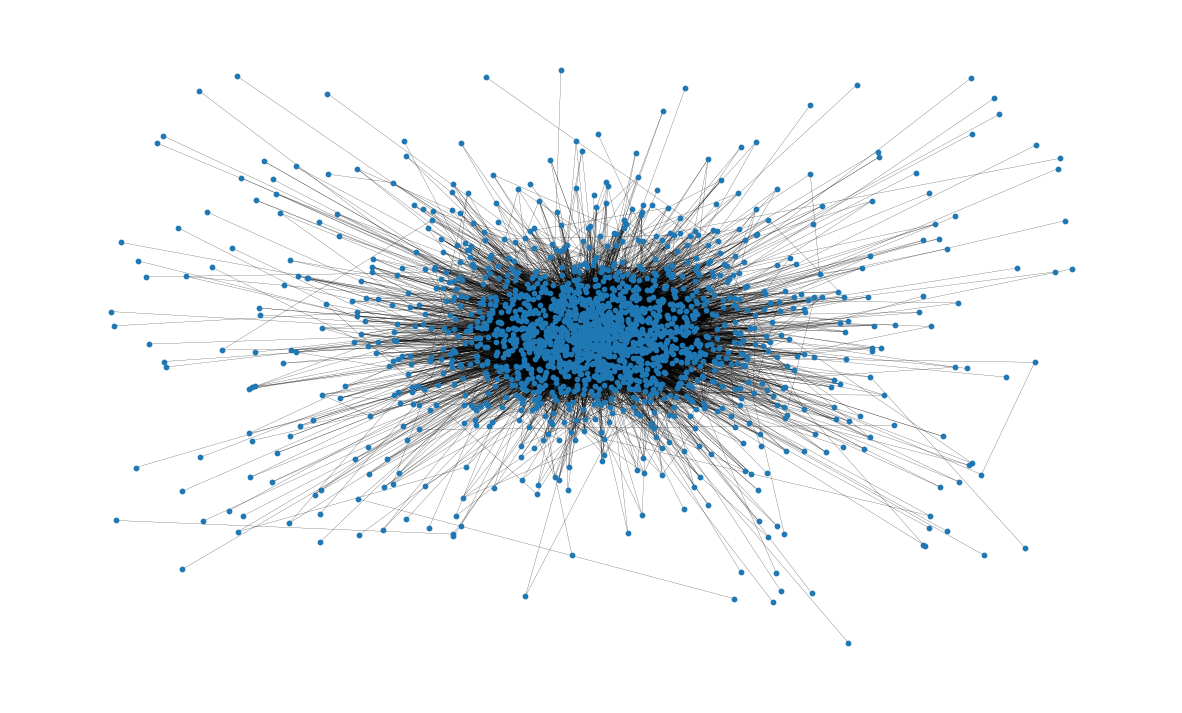
\includegraphics[width=0.6\textwidth]{assets/network_visual.png}
\caption{Brazilian Portuguese Twitch Streamers Social Network Visualization}
\label{fig:Network}
\end{figure}

This social network has an edge density of $1.71\%$ which is the ratio of actual
friendships compared to the maximum possible number of friendships. So, we can
say that this network is very sparse. The network consists of one (1) connected
component and has an average clustering coefficient of $31.99\%$ meaning that a
streamer's friends have on average around $32\%$ chance of being friends.
Streamers on average have almost $33$ friends; this is calculated as the average
degree of a node, which is $32.74\%$. The degree distribution in
\textit{figure \ref{fig:DegreeDist}} is a histogram that displays how many streamers
(\textit{number of nodes} on the y-axis) have a number of friends
(\textit{degree} on the x-axis).

\begin{figure}[H]
\centering
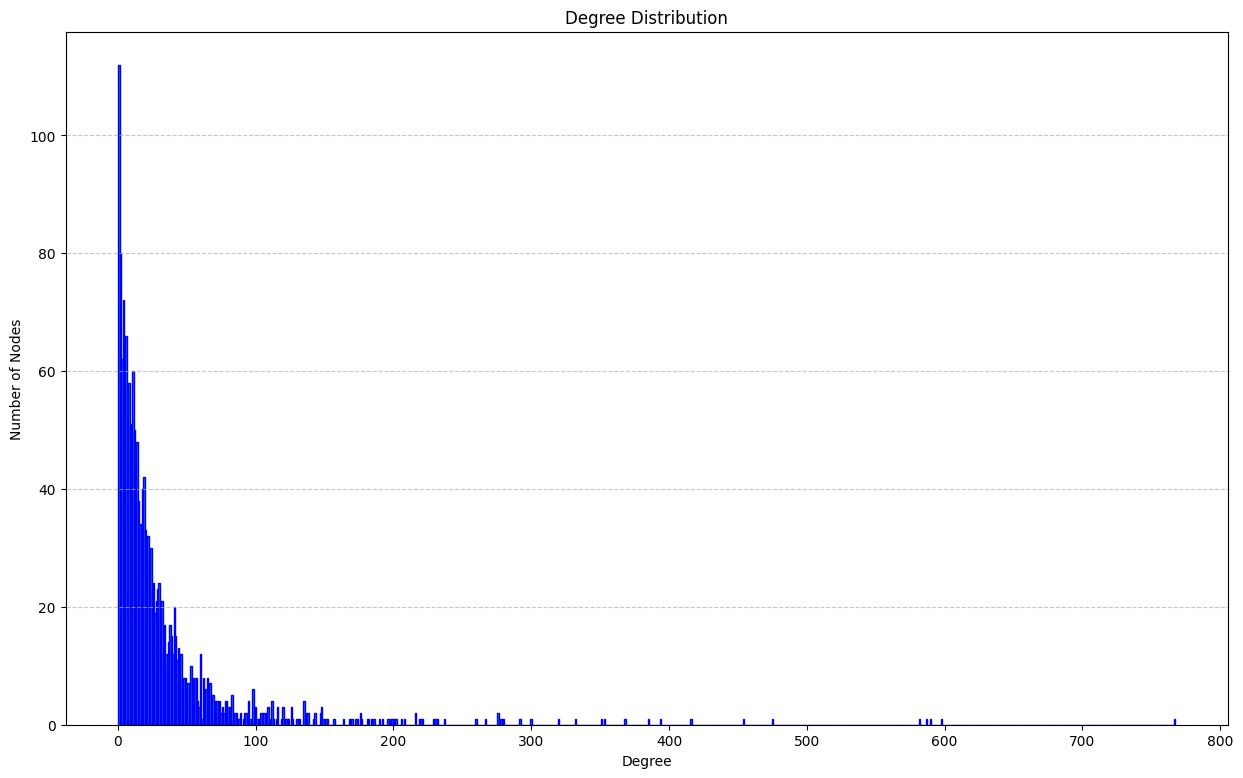
\includegraphics[width=0.6\textwidth]{assets/degree_dist.png}
\caption{Distribution of Number Twitch Streamers Friends}
\label{fig:DegreeDist}
\end{figure}

From the degree distribution, we can see that a lot of streamers have a small
amount of friends and towards the right side of the graph a few streamers have
a lot of friends. This distribution is very heavily skewed, which would follow
a \textit{power-law} distribution. These distributions have the property of
being scale-free and tend to have very heavy tails, leading them to be
referred to as the \textit{"80/20" rule} distribution. On average, a streamer
in this network is $3$ friendships away from another streamer. To obtain this
information, all the shortest paths from all streamers to all other streamers
are calculated and then averaged. The distribution of these shortest paths
\textit{figure \ref{fig:SP_Dist}} shows that even though being $2$ friends away
for non-connected streamers is more common; unconnected streamers are $3$
friends apart on average.

\begin{figure}[H]
\centering
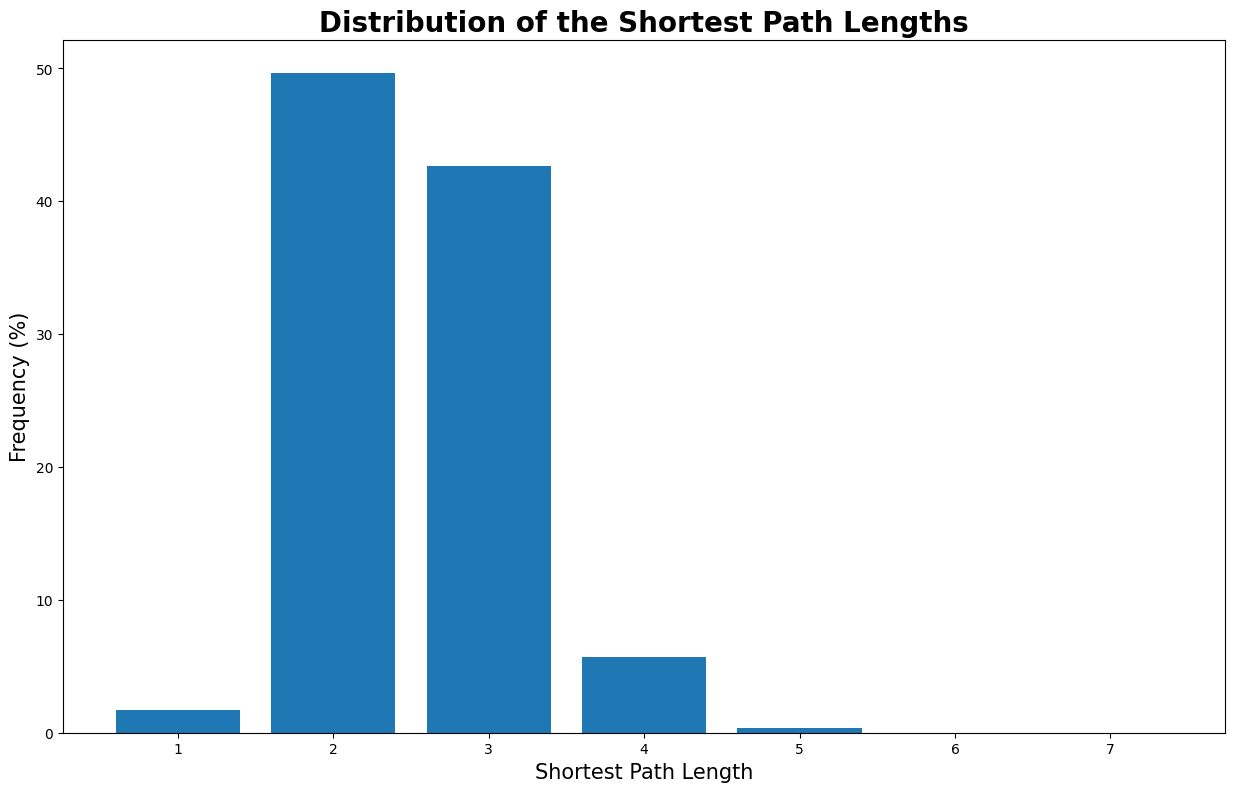
\includegraphics[width=0.6\textwidth]{assets/sp_dist.png}
\caption{Distribution of How Many Friends Are Between Non-Connected Streamers}
\label{fig:SP_Dist}
\end{figure}

Another piece of the histogram of the shortest path distribution above shows
that the maximum number of friends apart is $7$, which is the \textit{diameter}
of the network.


\subsection{Network Centralities and Communities}

The topic of \textit{centrality} is very important in graph theory and network analysis.
There are different centrality measures that help to explain the behavior of the
network. These measures of centrality in this \textit{Twitch} social network context
would include degree centrality (the number of direct friends a streamer has),
betweenness centrality (how many times a streamer is a friend in the shortest
path), closeness centrality (How close a streamer is to all the other streamers),
and eigenvector centrality (a streamer's influence on other important streamers).
Then we have the \textit{PageRank} algorithm, which in this context would tell us how
important a streamer is based on their connections to other streamers who have
a lot of friends or quality connections. In the \textit{table \ref{tab:centrality}}
below, which includes the top $10$ streamers for each centrality and the PageRank
algorithm.

\begin{table}[H]
\footnotesize
\centering
\begin{tabular}{|c|c|c|c|c|c|}
\hline
    \bf{Node} & \bf{Degree} & \bf{Betweenness} & \bf{Closeness}
    & \bf{Eigenvector} & \bf{PageRank} \\
\hline
    1 & 127 & 127 & 127 & 127 & 127 \\
    2 & 1476 & 1476 & 1297 & 1297 & 1476 \\
    3 & 290 & 1297 & 467 & 467 & 290 \\
    4 & 1297 & 290 & 290 & 290 & 1297 \\
    5 & 467 & 467 & 1476 & 1476 & 467 \\
    6 & 1660 & 67 & 67 & 1660 & 1660 \\
    7 & 67 & 1660 & 1660 & 67 & 67 \\
    8 & 1320 & 1259 & 1593 & 1593 & 1320 \\
    9 & 1758 & 287 & 1259 & 1320 & 1758 \\
    10 & 1259 & 428 & 287 & 1758 & 1259 \\
\hline
\end{tabular}
\caption{Top 10 Centrality and PageRank Measures}
\label{tab:centrality}
\end{table}

Looking through the measures, node $127$ is at the top of each measure.
Nodes $67, 290, 467, 1297, 1476$ and $1660$ appearing in the top $7$ of
each measure. Nodes $1320$ and $1758$ appear in the \textit{degree} and
the \textit{eigenvector} centralities and \textit{PageRank}, where node
$1259$ appears across all measures except for \textit{eigenvector}
centrality. Node $1593$ is in the top 10 for only the \textit{closeness}
and the \textit{eigenvector} centralities. Node $287$ is only in the top 10
for the \textit{betweeness} and the \textit{closeness} centralities. Finally,
node $428$ is only in the top 10 for the \textit{betweenness} centrality
across all the centralities and PageRank.

Another effective tool for analyzing the network centrality measures is
by visualizing the distribution of the centrality values for each measure
as in \textit{figure \ref{fig:cent_dist}}. These histograms will provide
valuable insight for the spread of the measure, the skewness of the
measure, and the ability to identify outliers.

\begin{figure}[H]
\centering
    \subfigure[]{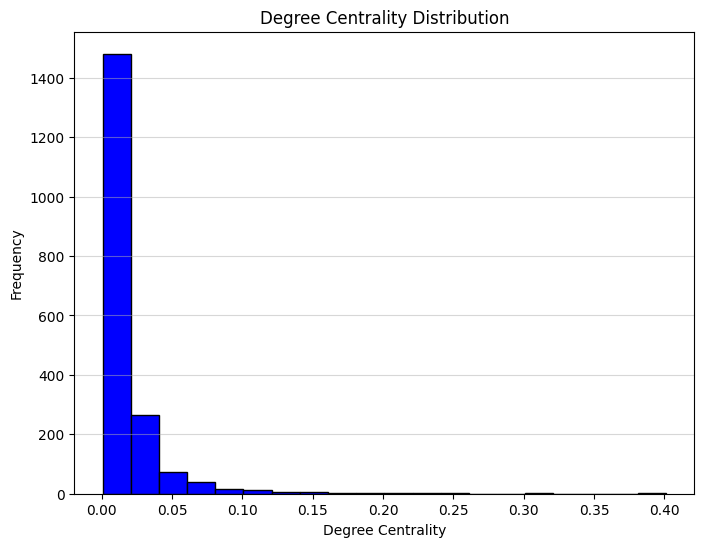
\includegraphics[width=0.28\textwidth]{assets/cent_dist_degree.png}}
    \subfigure[]{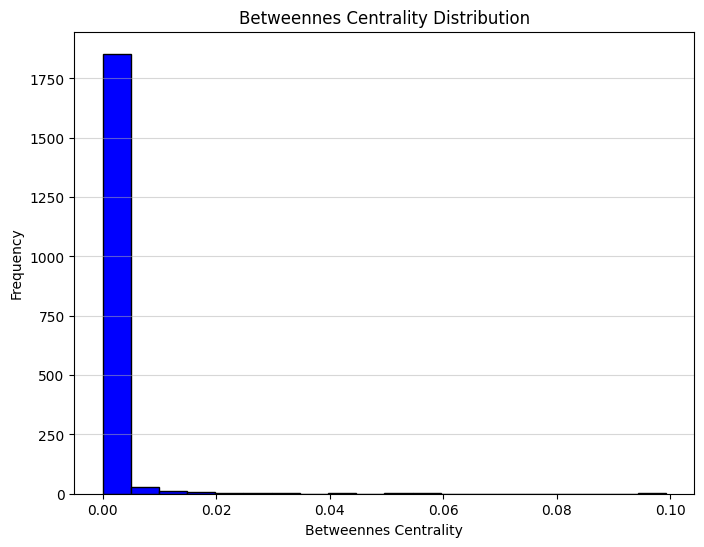
\includegraphics[width=0.28\textwidth]{assets/cent_dist_between.png}}
    \subfigure[]{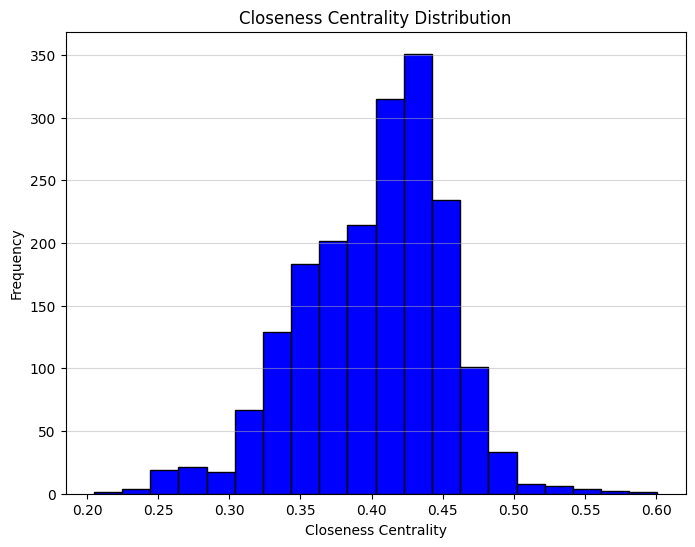
\includegraphics[width=0.28\textwidth]{assets/cent_dist_close.png}}
    \subfigure[]{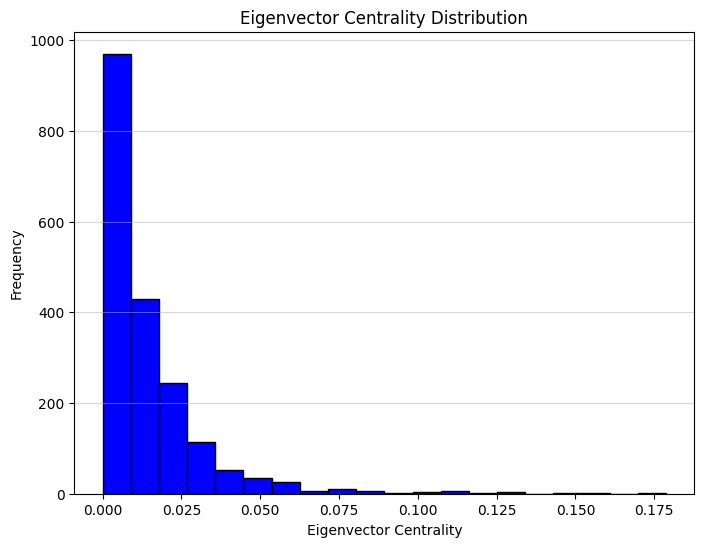
\includegraphics[width=0.28\textwidth]{assets/cent_dist_eigen.png}}
    \subfigure[]{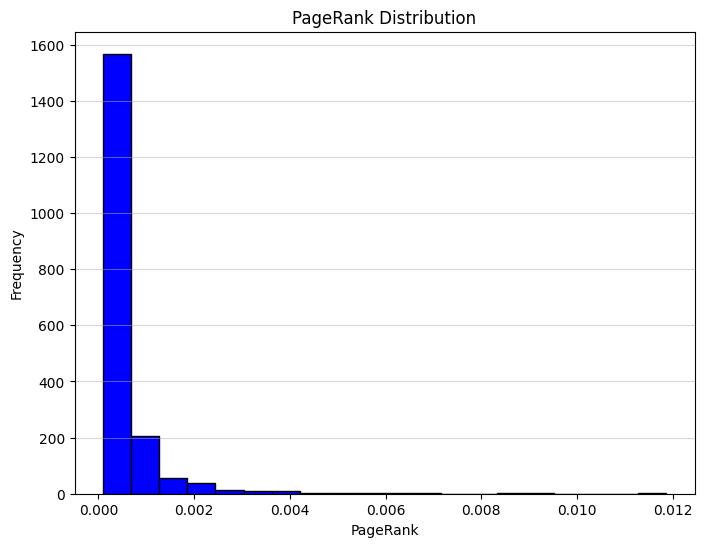
\includegraphics[width=0.28\textwidth]{assets/cent_dist_pr.png}}
\caption{
    Centrality Measures and PageRank Algorithm \\
    \footnotesize
    (a) Degree Centrality Histogram
    (b) Betweenness Centrality Histogram
    (c) Closeness Centrality Histogram
    (d) Eigenvector Centrality Histogram
    (e) PageRank Histogram
}
\label{fig:cent_dist}
\end{figure}

From the centrality measurement histograms above, we can see that there is
a skewness on all the measures except for the closeness centrality. There
appear to be outliers in each of the measures. The outliers and skewness of
centrality distributions will be further observed in the feature engineering
in part 2.

Communities in this network will provide insight into the groups of friends
where a streamer can only be part of one (1) group of friends. Using the
\textit{Louvain} method for community detection, we were able to detect
$6$ communities in this network. The communities' sizes are
$96, 374, 485, 304, 437$ and $216$. The next step was to attach viewing
behavior attributes to each streamer. Then we were able to see the average
behavior of each community in \textit{table \ref{tab:comm_att}}.

\begin{table}[H]
\footnotesize
\centering
\begin{tabular}{|c|c|c|c|c|}
\hline
    \bf{Community} & \bf{Community Size} & \bf{Average Views}
     & \bf{Per Day} & \bf{Average Per Day} \\
\hline
    1 & 96 & 293829.4792 & 166889 & 1738.4271 \\
    2 & 374 & 212264.2540 & 457668 &  1223.7112 \\
    3 & 485 & 272537.9340 & 675075 & 1391.9072 \\
    4 & 304 & 1291529.8487 & 402944 & 1325.4737 \\
    5 & 437 & 308141.0366 & 485237 & 1110.3822 \\
    6 & 216 &  66690.7917 & 350209 & 1621.3380 \\
\hline
\end{tabular}
\caption{Community Average Viewing}
\label{tab:comm_att}
\end{table}

Looking at the table above to compare communities.
Community $1$ with $96$ streamers accounts is the smallest community with
$12.02\%$ of average views, but has the highest average per day with around
$20.67\%$. This group accounts for $6.58\%$ of days.
Community $2$ with $374$ streamers has one of the lowest average views with a
third largest community at $8.68\%$, and has the second lowest per day with
$14.56\%$. This group accounts for $18.03\%$ of days.
Community $3$ with $485$ streamers is the largest community. The views and per day
averages are in the middle of the pack with $11.15\%$ and $16.55\%$
respectively. This group accounts for $26.60\%$ of days.
Community $4$ with $304$ streamers leads average views by a massive margin with
$52.82\%$ of all views, but has less average per day than communities $1, 3$
and $6$ with only around $15.88\%$. This group accounts for $18.03\%$ of days.
Community $5$ with $437$ streamers is the second largest community with an average
$12.60\%$ of all views but has the lowest average per day with only
$13.20\%$. This group represents $19.12\%$ of days.
Community $6$ with $216$ streamers is the second smallest community, and has the
lowest average views with only $2.73\%$ of all views but has the second
highest average per day with around $19.28\%$. This group accounts for
$13.80\%$ of days.
So, from the table and information above, communities'
$1$ and $6$ have the highest per day average in their community. Community $4$
leads with the most views from a smaller user pool, and community $3$ with the
largest user group lead for per day usage, but only the third highest average
per day usage.


\section{Part 2 - Predictive Modeling}

The goal of the predictive modeling portion, is to build a model
with \textbf{Logistic Regression} model to predict the target state
of whether a streamer is partnered or non-partnered. Using feature
engineering based on the EDA in part 1, we will examine the features
from the graph measures and viewing behavior to build a model
after treating the data to predict a streamer's partnership, and
then evaluate the model's performance.

\subsection{Feature Engineering}

From the EDA in part 1, predictive features will be used from both
the network measures and viewing behavior attributes. The features
for this model will either be numerical or nominal, which is a
categorical feature that has no inherent order. All the features
selected from the network measures are numerical. The selected
network features are centralities for \textit{Degree, Betweenness,}
\textit{Closeness, Eigenvector,} and the \textit{PageRank} algorithm.
The selected features from the viewing behavior attributes include
\textit{Days} and \textit{Views} as numerical features, and
\textit{Mature Content} as a nominal categorical feature.
\textit{Figure \ref{fig:features}} displays the engineered features
with boxplots for the numerical features and bar charts for the
categorical feature.

\begin{figure}[H]
\centering
    \subfigure[]{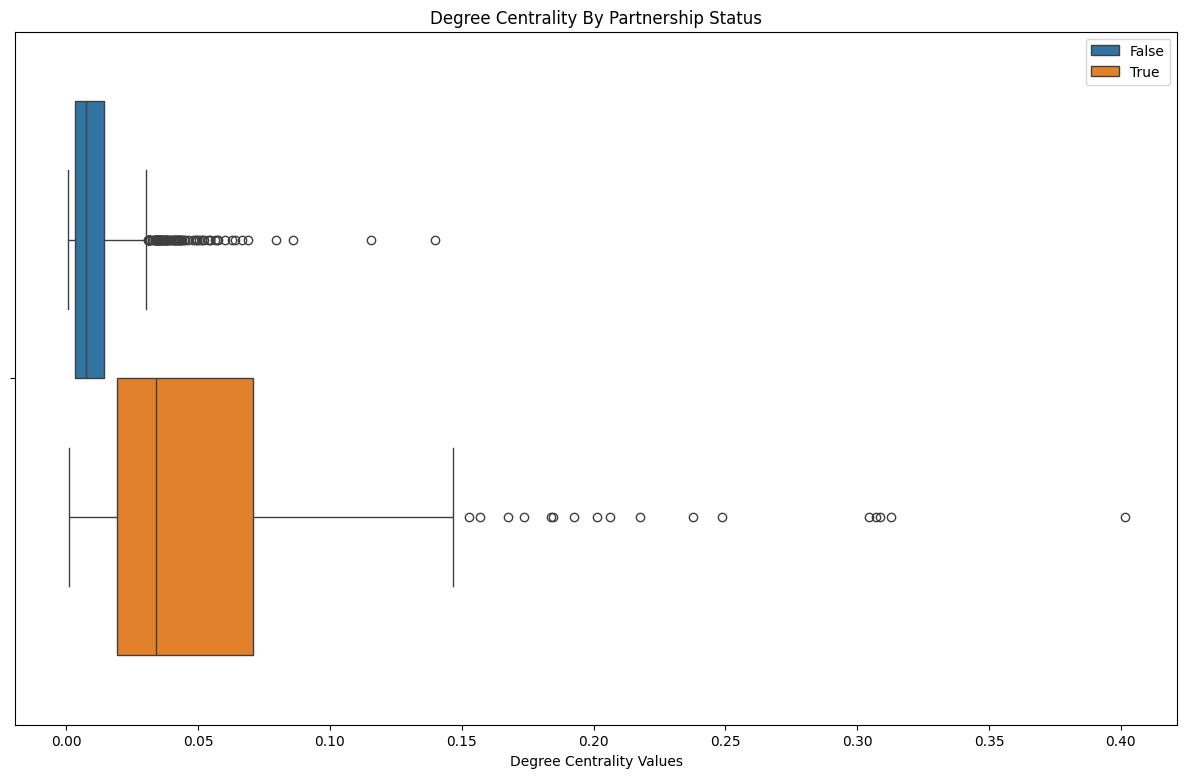
\includegraphics[width=0.28\textwidth]{assets/deg_feat.png}}
    \subfigure[]{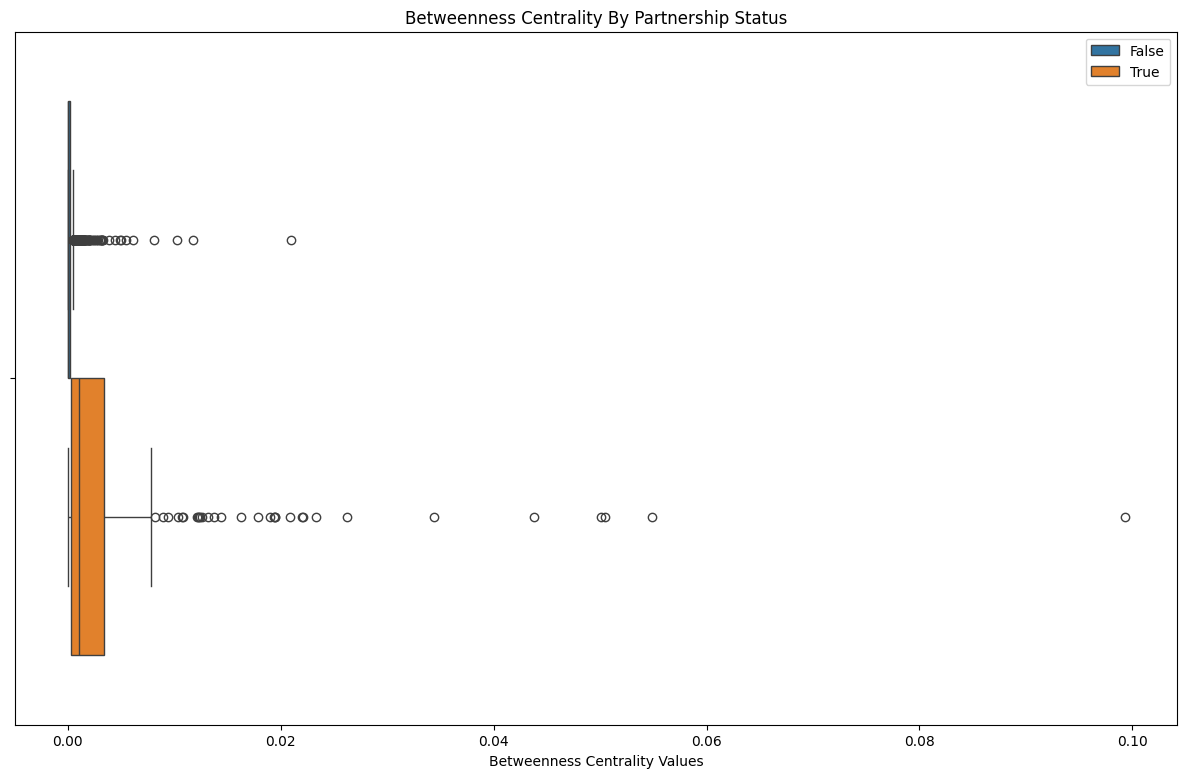
\includegraphics[width=0.28\textwidth]{assets/bet_feat.png}}
    \subfigure[]{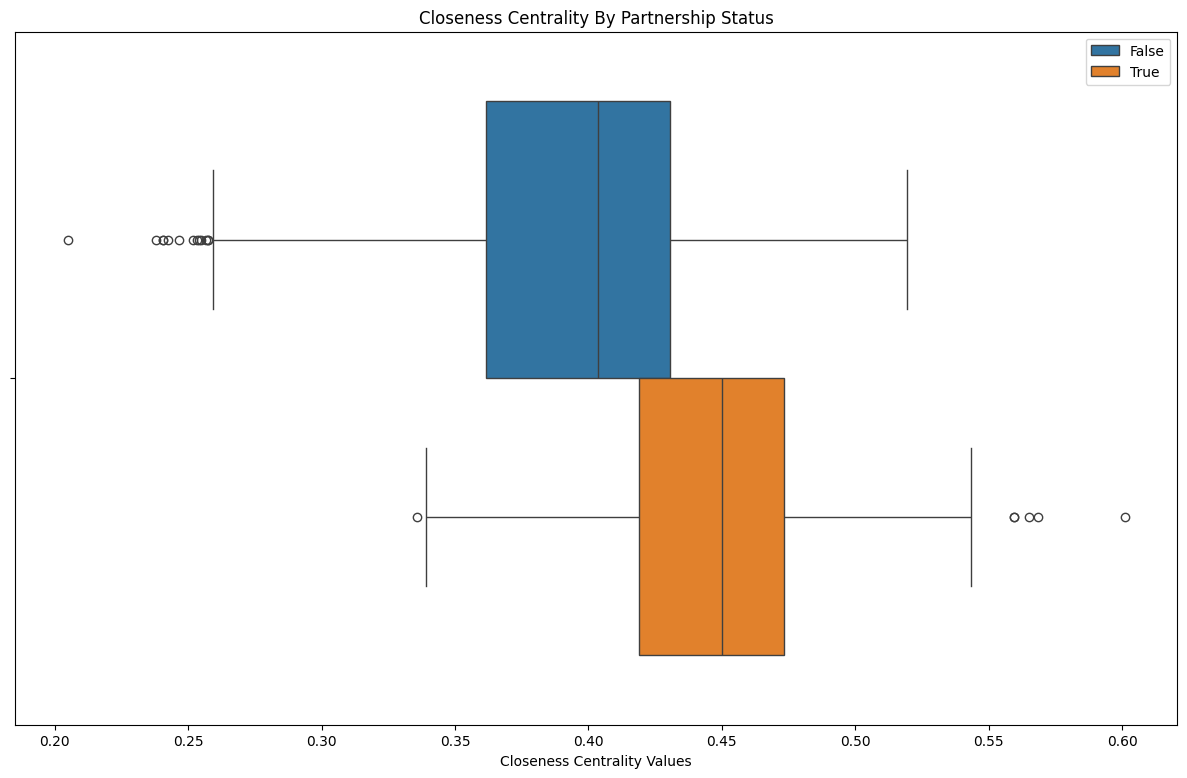
\includegraphics[width=0.28\textwidth]{assets/close_feat.png}}
    \subfigure[]{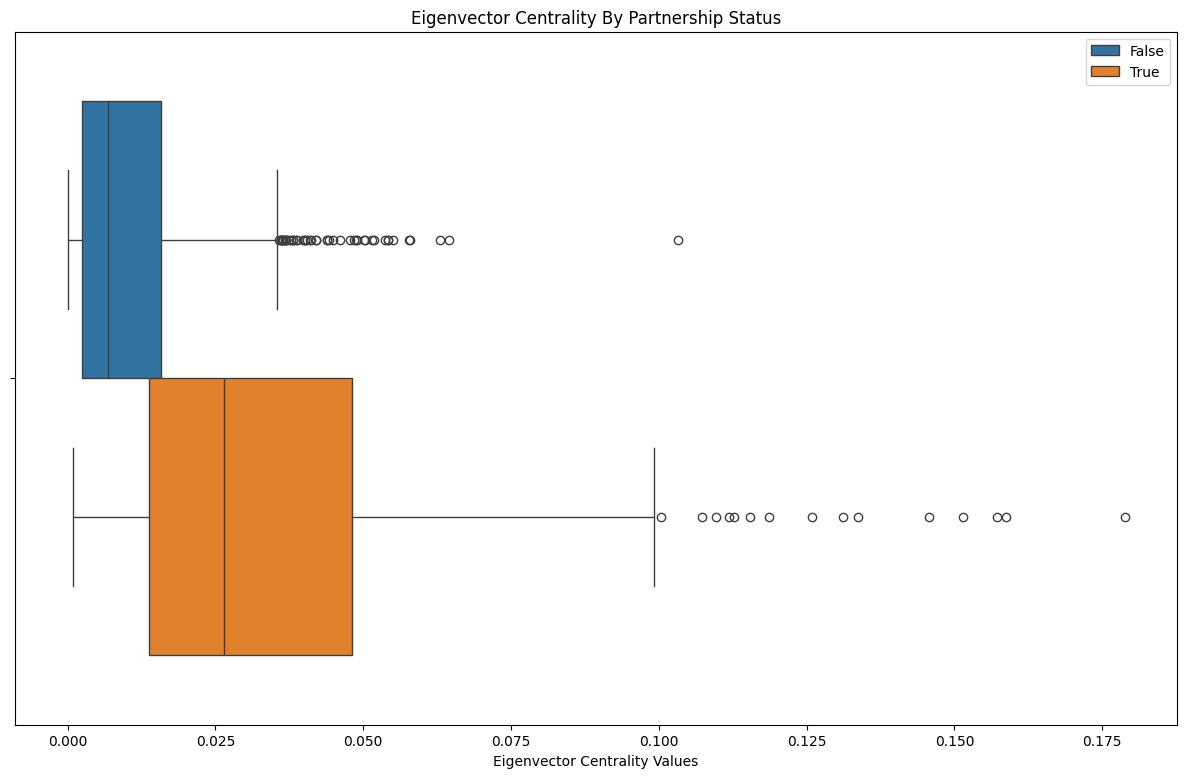
\includegraphics[width=0.28\textwidth]{assets/eigen_feat.png}}
    \subfigure[]{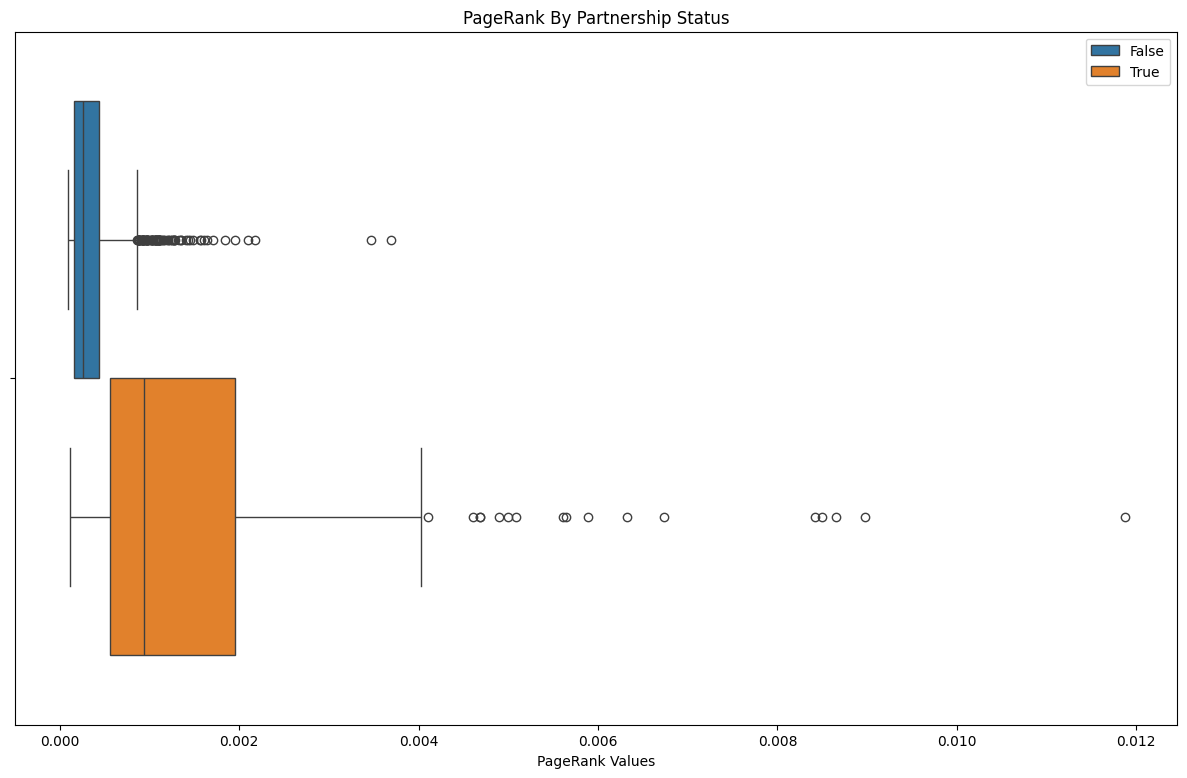
\includegraphics[width=0.28\textwidth]{assets/pr_feat.png}}
    \subfigure[]{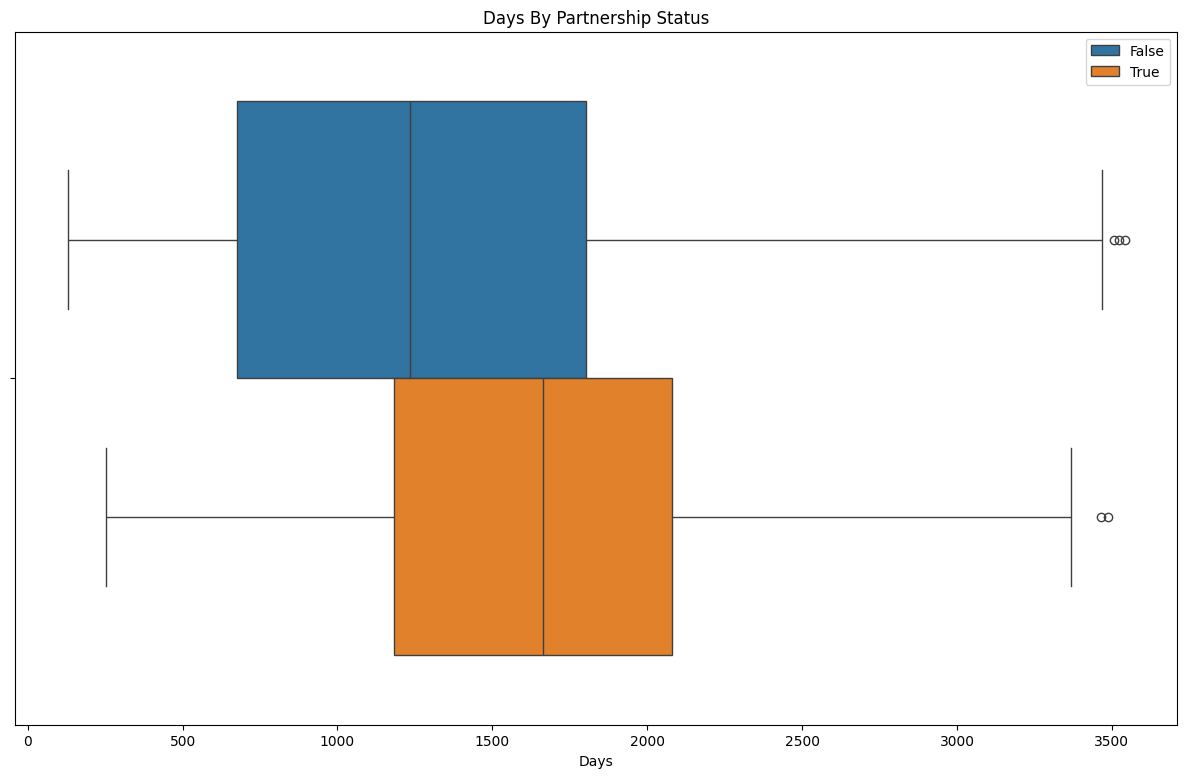
\includegraphics[width=0.28\textwidth]{assets/days_feat.png}}
    \subfigure[]{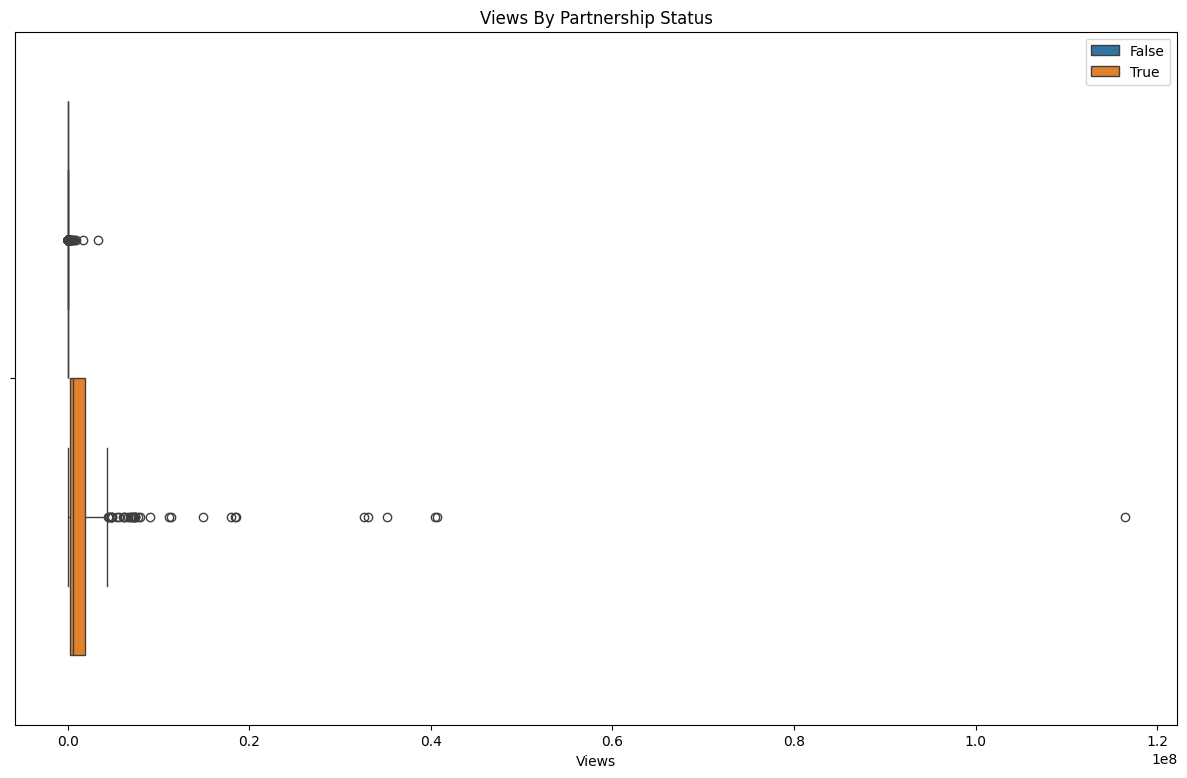
\includegraphics[width=0.28\textwidth]{assets/views_feat.png}}
    \subfigure[]{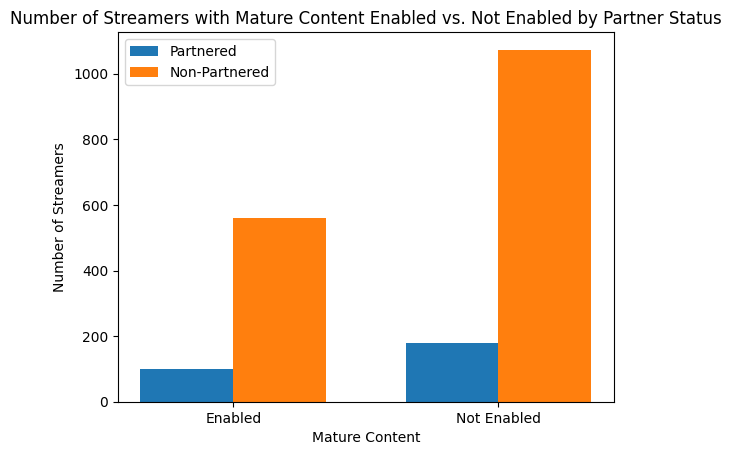
\includegraphics[width=0.28\textwidth]{assets/mature_feat.png}}
\caption{
    Modeled Features Visualizations \\
    \footnotesize
    (a) Degree Centrality Feature
    (b) Betweenness Centrality Feature
    (c) Closeness Centrality Feature
    (d) Eigenvector Centrality Feature
    (e) PageRank Feature
    (f) Days Feature
    (g) Views Feature
    (h) Mature Content Feature
}
\label{fig:features}
\end{figure}

Looking at the selected features in the above visualizations,
\textit{Closeness, Eigenvector} centralities, \textit{PageRank},
\textit{Days}, and \textit{Views} numerical features, and
\textit{Mature Content} categorical feature appear to be the important
features in the predictive model.
The partnered streamers have a lot more direct friendship than the
non-partnered streamers. From the boxplot for \textit{degree centrality}
the largest outlier in the non-partnered streamers would not be an outlier
among the partnered streamers, and a majority of the non-partnered outliers
would fall below the third quartile $Q3$ of the partnered streamer group.
From the boxplot for \textit{betweenness centrality} the partnered streamers are
more important connecting to other user than the non-partnered streamers even
though the betweenness in either group is not large.
The \textit{closeness centrality} boxplot shows that partnered streamers have a
greater ability to reach other users than the non-partnered streamers.
The \textit{Eigenvector centrality} boxplot shows that partnered streamers are more
influential than non-partnered streamers. The maximum and a majority of the
non-partnered streamers outliers still fall below the third quartile $Q3$ of
the partnered streamers showing us that partnered streamers are influential.
The \textit{PageRank} boxplot shows us that partnered streamers are more important to
the friendships in the network than non-partnered streamers. Again, this is
very heavily favored towards partnered streamers against non-partnered
streamers.

The dataset is comprised of $1,633$ non-partnered streamer and $279$ partnered
streamers. The non-partnered streamers make up about $85.4\%$ of the data.
So, there is a large imbalance in the dataset for the partner
class that favors the non-partnered streamers. To handle the class
imbalance, a sampling method was applied to the majority class to randomly
select an amount of data similar to the minority class for model evaluation.
This is an important part of modeling to prevent overfitting of the model.
The \textit{table \ref{tab:class_imb}} and \textit{figure \ref{fig:class_imb}}
show the before and after the sampling method was applied.

\begin{table}[H]
\footnotesize
\centering
\begin{tabular}{l c|c}
\hline
    \bf{Class} & \bf{Imbalanced Dataset} & \bf{Balanced Dataset} \\
\hline
    Partnered: & 279 & 279 \\
    Non-Partnered: & 1633 & 294 \\
\hline
\end{tabular}
\caption{Comparing Target Class Imbalance}
\label{tab:class_imb}
\end{table}

\begin{figure}[H]
\centering
    \subfigure[]{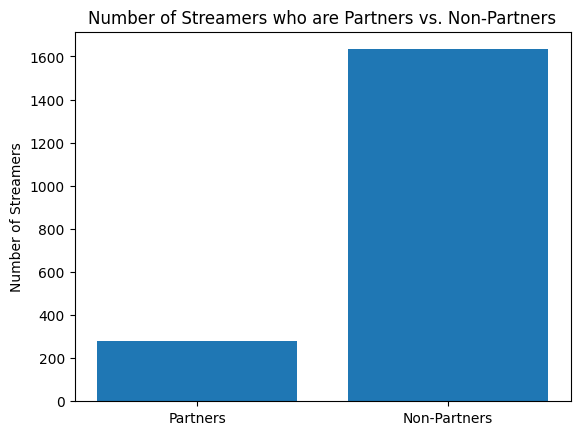
\includegraphics[width=0.34\textwidth]{assets/class_imbalance.png}}
    \subfigure[]{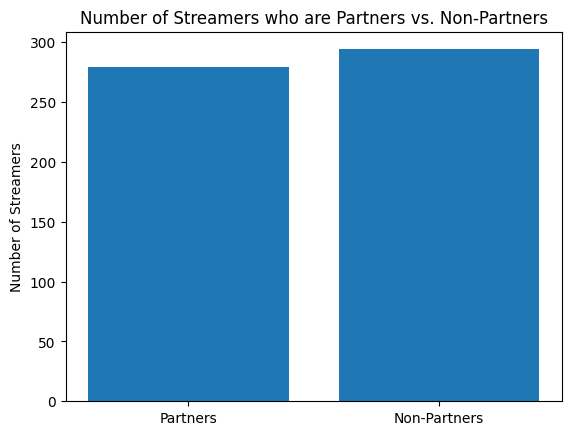
\includegraphics[width=0.34\textwidth]{assets/class_balance.png}}
\caption{
    Target Class Imbalance Visualization \\
    \footnotesize
    (a) - Original Imbalanced Dataset
    (b) - Sampled Balanced Dataset
}
\label{fig:class_imb}
\end{figure}

\subsection{Training And Evaluation}

Now the feature engineering is finished, one more dataset adjustments
is needed. The target column \textit{Partner} has to be converted to
a numerical value from it \textit{True/False} boolean state. Then,
the dataset will be randomly split into a training and test datasets
with around $80\%$ of the balanced dataset being assigned to the training
set and around $20\%$ assigned to the test set shown in
\textit{table \ref{tab:tt_set}}.

\begin{table}[H]
\footnotesize
\centering
\begin{tabular}{l c}
\hline
    {} & \bf{Dataset Size} \\
\hline
    Training Set: & 453 \\
    Test Set: & 120 \\
\hline
\end{tabular}
\caption{Training and Test Set Sizes}
\label{tab:tt_set}
\end{table}

Using a \textbf{Logistic Regression} model along with the more common
evaluation metrics for classification (\textit{Precision, Recall, Accuracy}
and \textit{F1 Score}) in \textit{eq \ref{eq:bg}, \ref{eq:acc},\ref{eq:f1}},
a predictive model will be trained and evaluated initial using a
\textbf{k-folds} cross-validation.

\tiny
\begin{equation}
\begin{split}
TP = True\ Positive \\
TN = True\ Negative \\
FP = False\ Positive \\
FN = False\ Negative \\
Precision = \frac{TP}{TP + FP} \\
Recall = \frac{TN}{TN + FP} \\
\end{split}
\label{eq:bg}
\end{equation}

\begin{equation}
Accuracy = \frac{FP}{TP + FP} = 1 - \frac{TP}{TP + FP}
\label{eq:acc}
\end{equation}

\begin{equation}
F_1\ Score = 2 * \frac{precision * recall}{precision + recall}
\label{eq:f1}
\end{equation}
\normalsize

This initial phase will fold the training dataset into $5$ folds
with around $20\%$ of the data assigned to a fold. Then, a process of
fitting $5$ logistic regression models with $4$ folds being used for training
and $1$ fold being used as the validation set will run until all k-folds
sets have been used as the validation set. Now, the evaluation metrics
from the validation sets across the 5 model will be averaged to compute
the training-validation metrics shown in \textit{table \ref{tab:k_folds}}.

\begin{table}[H]
\footnotesize
\centering
\begin{tabular}{l c}
\hline
    {} & \bf{Evaluation Metric} \\
\hline
    Accuracy: & 90.3460 \\
    F1 Score: & 0.9033 \\
    Precision: & 0.8770 \\
    Recall: & 0.9547 \\
\hline
\end{tabular}
\caption{K-Folds Evaluation Metrics}
\label{tab:k_folds}
\end{table}

Since the \textbf{k-folds} cross-validation produced an acceptable performance
on the validation, we will now train the model on the full training
dataset and test the model performance with evaluation metrics,
which are shown in \textit{table \ref{tab:final_model}}

\begin{table}[H]
\footnotesize
\centering
\begin{tabular}{l c}
\hline
    {} & \bf{Evaluation Metric} \\
\hline
    Accuracy: & 90.8333\\
    F1 Score: & 0.90817 \\
    Precision: & 0.8769 \\
    Recall: & 0.9500 \\
\hline
\end{tabular}
\caption{Final Model Evaluation Metrics}
\label{tab:final_model}
\end{table}

The average metrics for Precision and Recall were slightly higher for the
k-folds cross-validation. The final model that was trained on the full
training set outperformed the k-folds cross-validation method on Accuracy
and the F1 score. This might be due to the small sample size once the class
imbalance was handled. The most important predictive features were
\textit{PageRank} and  \textit{Eigenvector} centrality.
\textit{Days} and \textit{Views}  had little to no impact on the model.
\textit{Degree, Betweenness, Closeness} centralities and
\textit{Mature Content} had a negative impact on the model. The feature
importance is shown in \textit{table \ref{tab:feat_imp}}.

\begin{table}[H]
\footnotesize
\centering
\begin{tabular}{l c}
\hline
    {} & \bf{Feature Importance} \\
\hline
    Degree Centrality: & -315.9713 \\
    Betweenness Centrality: & -525.7118 \\
    Closeness Centrality: & -3.5342 \\
    Eigenvector Centrality: & 22.6962 \\
    PageRank: & 15653.5683 \\
    Days: & 0.0002 \\
    Mature Content: & -0.4519 \\
    Views: & 0.0 \\
\hline
\end{tabular}
\caption{Final Model Predictive Feature Importance}
\label{tab:feat_imp}
\end{table}

The logistic regression predictive model showed decent
performance on the balanced dataset. I would recommend
transforming the numerical features to attempt to increase
feature importance or remove them from the model.
I would also recommend transforming the categorical feature
\textit{Mature Content} to an ordinal feature to detect
streamers age or mature.


\section{Discussion}

\subsection{Compare and Contrast}

The graph measures, features, and data splits in both parts
of the project maintained consistency due to the seed being
set for repeatability.

In contrast and possibly as an extension to the project, it
would be an interesting experiment to use the current target
\textit{Partnership} as a feature and try to predict the
target state of a streamer's \textbf{Mature Content} rating.
As these were the two (2) categorical attributes.

\subsection{Limitations}
Due to the dataset class imbalance, much of the data was not able to be used
in the predictive modeling. This also had an impact on the feature engineering
phase for normalizing the numerical features.

\subsection{Extensions}

While modeling the features, the numerical feature \textit{views} has
a major skewness. In order to fix this, I ran the model with a
\textbf{Log Transformation} $log(x+1)$ applied to the
\textit{views} feature shown in
\textit{figures \ref{fig:log_dist} and \ref{fig:log_views_feat}}

\begin{figure}[H]
\centering
    \subfigure[]{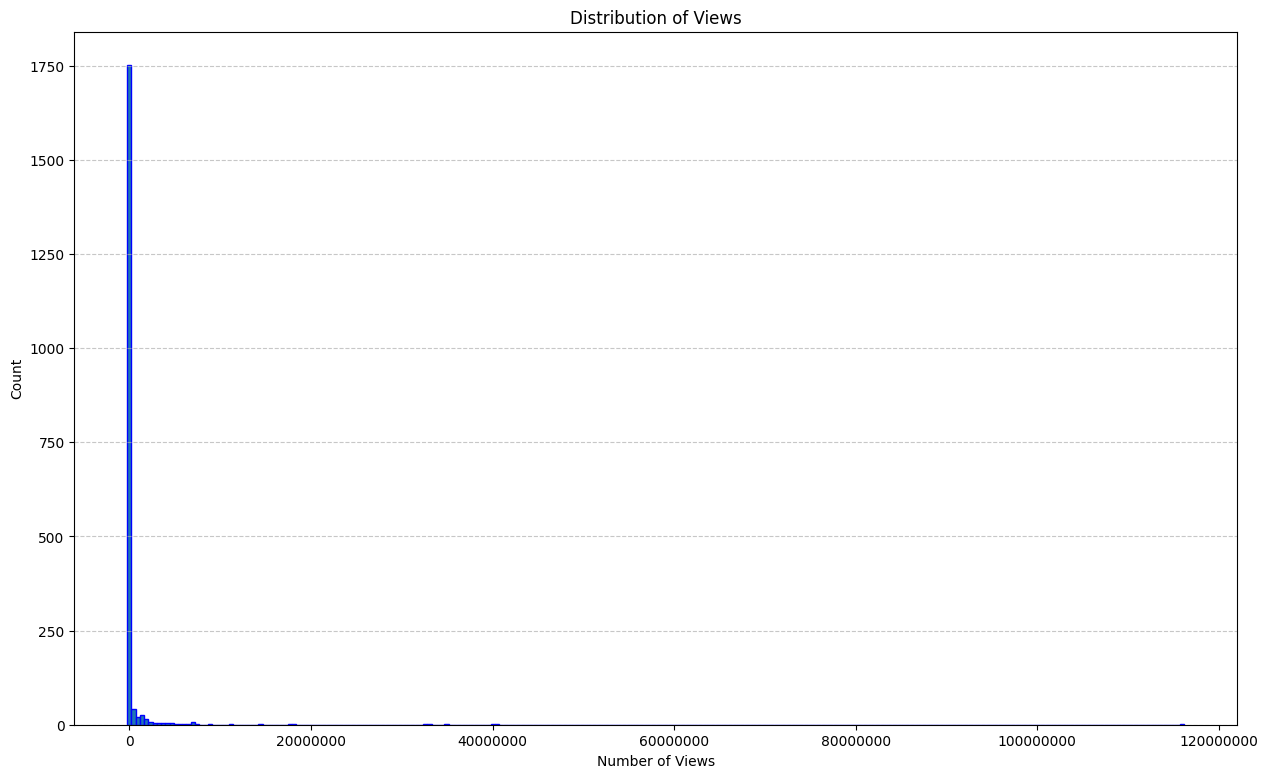
\includegraphics[width=0.45\textwidth]{assets/view_dist.png}}
    \subfigure[]{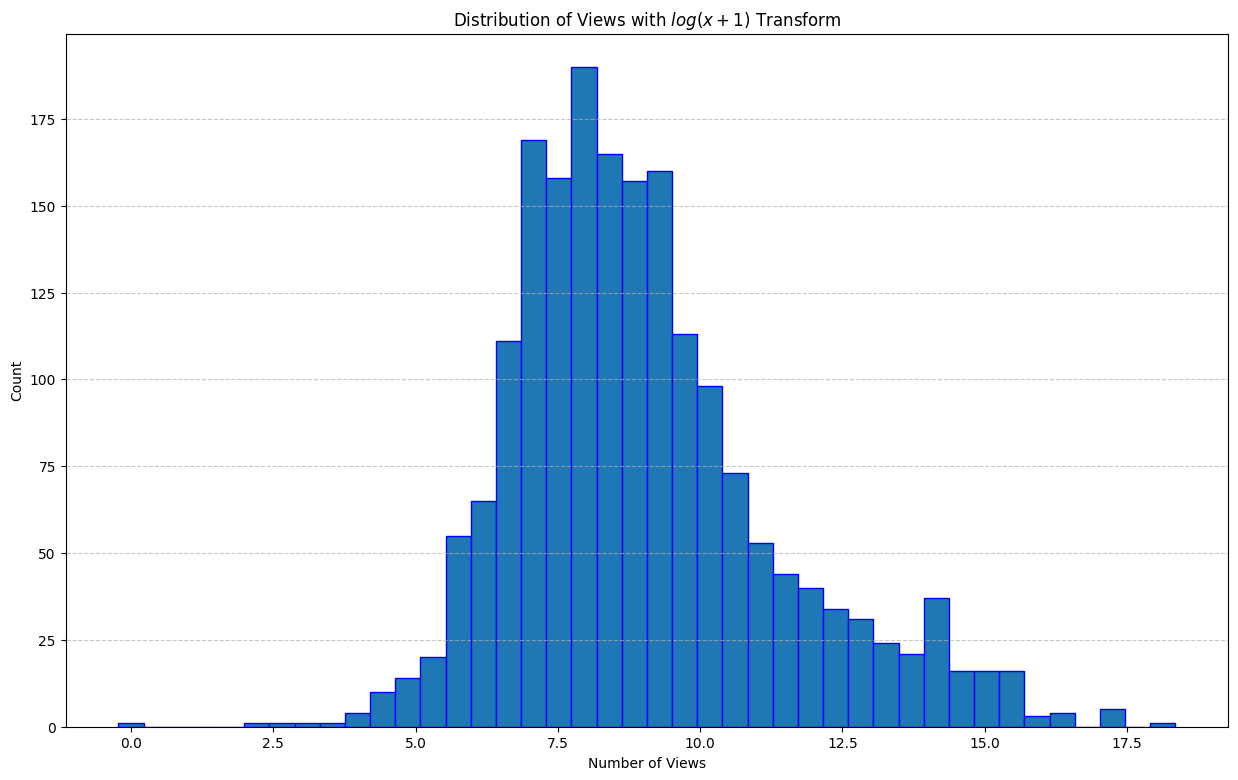
\includegraphics[width=0.45\textwidth]{assets/log_view_dist.png}}
\caption{
    Comparison of Views Feature Visualization \\
    \footnotesize
    (a) Original Views Data
    (b) Transformed Views Data
}
\label{fig:log_dist}
\end{figure}

\begin{figure}[H]
\centering
    \subfigure[]{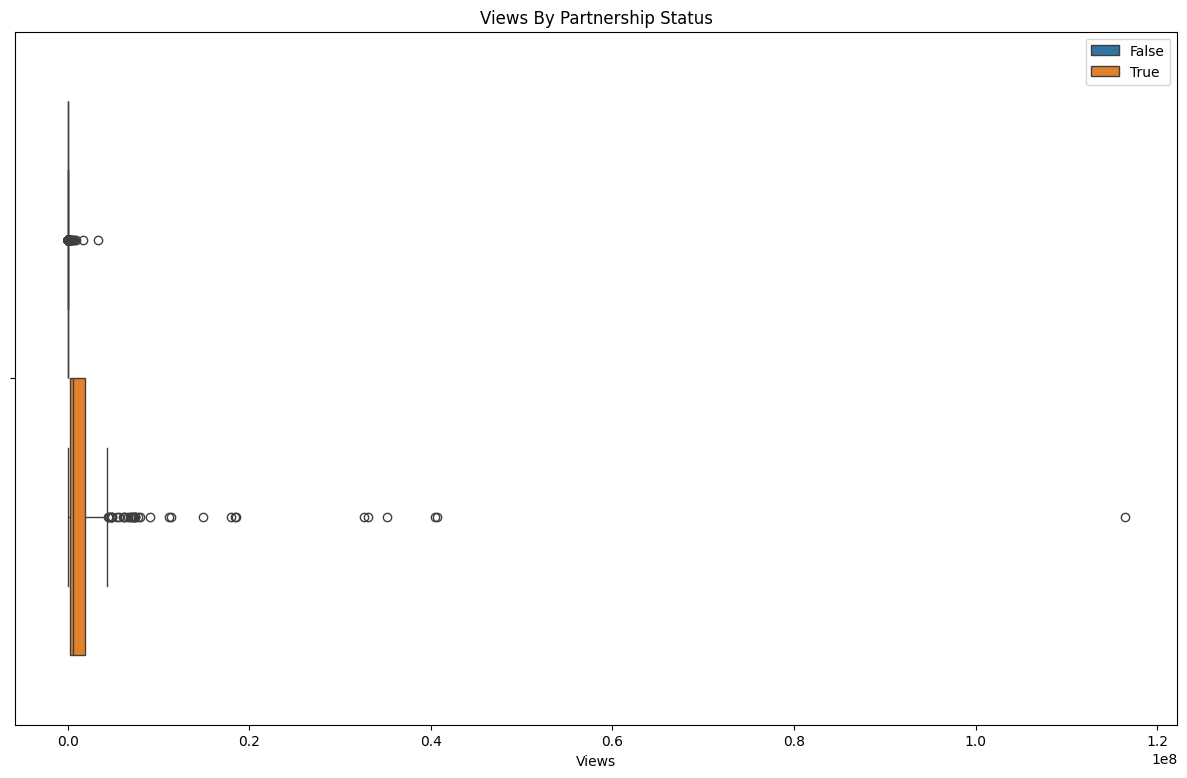
\includegraphics[width=0.45\textwidth]{assets/views_by_partner.png}}
    \subfigure[]{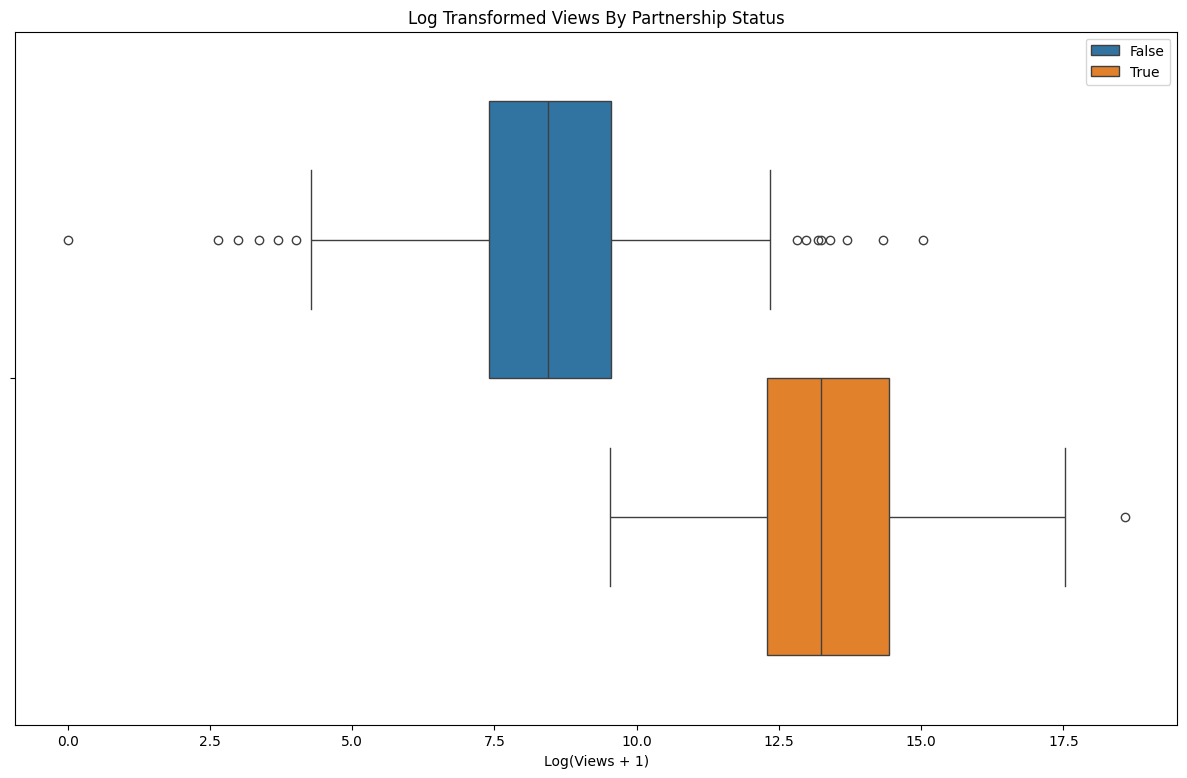
\includegraphics[width=0.45\textwidth]{assets/log_views_by_partner.png}}
\caption{
    Comparison of Views Feature By Partner Class \\
    \footnotesize
    (a) Original Views Feature
    (b) Transformed Views Feature
}
\label{fig:log_views_feat}
\end{figure}

The \textit{table \ref{tab:log_model} and \ref{tab:log_feat_imp}} has the result
compared to the original model in \textbf{Part 2} section.

\begin{table}[H]
\footnotesize
\centering
\begin{tabular}{l c|c}
\hline
    \bf{Evaluation Metric} & \bf{Original Model} & \bf{New Model} \\
\hline
    Accuracy: & 90.8333 & 96.6667 \\
    F1 Score: & 0.90817 & 0.9667 \\
    Precision: & 0.8769 & 0.9828 \\
    Recall: & 0.9500 & 0.9500 \\
\hline
\end{tabular}
\caption{Comparing Original Model to Transformed Model}
\label{tab:log_model}
\end{table}

\begin{table}[H]
\footnotesize
\centering
\begin{tabular}{l c|c}
\hline
    \bf{Feature Importance} & \bf{Original Model} & \bf{New Model} \\
\hline
    Degree Centrality: & -315.9713 & -340.4556 \\
    Betweenness Centrality: & -525.7118 & -264.0899 \\
    Closeness Centrality: & -3.5342 & -10.7687 \\
    Eigenvector Centrality: & 22.6962 & 104.7714 \\
    PageRank: & 15653.5683 & 13093.0474 \\
    Days: & 0.0002 & 0.0003\\
    Mature Content: & -0.4519 & -0.8946 \\
    Views: & 0.0 & 1.9931 \\
\hline
\end{tabular}
\caption{Comparing Final Model and Transformed Model Feature Importance}
\label{tab:log_feat_imp}
\end{table}

After looking at the performance, I would suggest as an
extension of this project would be to normalize the other
numerical features with the same transformation.
I would also recommend transforming the categorical feature
\textit{Mature Content} to an ordinal feature to detect streamers
age or mature.


\section{Conclusion}

In this project, we have explored the use of network structures
with basic graph measures, centrality, and communities. We
demonstrated how to build predictive models through feature
engineering and machine learning to classify a streamer's
attributes. We evaluated the models with the common metrics
for classification and diagnosed the features based on their
importance. The results of the model are decent, but the
extend work shows that more feature engineering and selection
can be done to improve the models performance.

\section{Project Links}
\large
\begin{itemize}
    \item \href{https://snap.stanford.edu/data/twitch-social-networks.html}
    {Twitch Social Network Dataset}
    \item \href{https://github.com/jmwinemiller/cap-6315-project}
    {Project GitHub}
    \item \href{https://colab.research.google.com/drive/1PBR3qY-72iEfz-Xa9Fxx154dKrOsx_8-}
    {Google Colab - Project Part 1}
    \item \href{https://colab.research.google.com/drive/1qGJSBkJfJrQsiWbSuAR0w9ISzZR-hiyj}
    {Google Colab - Project Part 2}
    \item \href{https://www.overleaf.com/read/xrsbhmvfwvqc#2ab9ba}
    {Overleaf Report}
\end{itemize}
\end{document}